\iffalse
\let\negmedspace\undefined
\let\negthickspace\undefined
\documentclass[journal,12pt,onecolumn]{IEEEtran}
\usepackage{cite}
\usepackage{amsmath,amssymb,amsfonts,amsthm}
%\usepackage{algorithmic}
\usepackage{graphicx}
\usepackage{textcomp}
\usepackage{xcolor}
\usepackage{txfonts}
\usepackage{listings}
\usepackage{enumitem}
\usepackage{mathtools}
\usepackage{gensymb}
\usepackage[breaklinks=true]{hyperref}
\usepackage{tkz-euclide} % loads  TikZ and tkz-base
\usepackage{listings}
\usepackage{float}



\newtheorem{theorem}{Theorem}[section]
\newtheorem{problem}{Problem}
\newtheorem{proposition}{Proposition}[section]
\newtheorem{lemma}{Lemma}[section]
\newtheorem{corollary}[theorem]{Corollary}
\newtheorem{example}{Example}[section]
\newtheorem{definition}[problem]{Definition}
%\newtheorem{thm}{Theorem}[section] 
%\newtheorem{defn}[thm]{Definition}
%\newtheorem{algorithm}{Algorithm}[section]
%\newtheorem{cor}{Corollary}
\newcommand{\BEQA}{\begin{eqnarray}}
\newcommand{\EEQA}{\end{eqnarray}}
\newcommand{\define}{\stackrel{\triangle}{=}}
\theoremstyle{remark}
\newtheorem{rem}{Remark}
%\bibliographystyle{ieeetr}
\begin{document}
%
\providecommand{\pr}[1]{\ensuremath{\Pr\left(#1\right)}}
\providecommand{\prt}[2]{\ensuremath{p_{#1}^{\left(#2\right)} }}        % own macro for this question
\providecommand{\qfunc}[1]{\ensuremath{Q\left(#1\right)}}
\providecommand{\sbrak}[1]{\ensuremath{{}\left[#1\right]}}
\providecommand{\lsbrak}[1]{\ensuremath{{}\left[#1\right.}}
\providecommand{\rsbrak}[1]{\ensuremath{{}\left.#1\right]}}
\providecommand{\brak}[1]{\ensuremath{\left(#1\right)}}
\providecommand{\lbrak}[1]{\ensuremath{\left(#1\right.}}
\providecommand{\rbrak}[1]{\ensuremath{\left.#1\right)}}
\providecommand{\cbrak}[1]{\ensuremath{\left\{#1\right\}}}
\providecommand{\lcbrak}[1]{\ensuremath{\left\{#1\right.}}
\providecommand{\rcbrak}[1]{\ensuremath{\left.#1\right\}}}
\newcommand{\sgn}{\mathop{\mathrm{sgn}}}
\providecommand{\abs}[1]{\left\vert#1\right\vert}
\providecommand{\res}[1]{\Res\displaylimits_{#1}} 
\providecommand{\norm}[1]{\left\lVert#1\right\rVert}
%\providecommand{\norm}[1]{\lVert#1\rVert}
\providecommand{\mtx}[1]{\mathbf{#1}}
\providecommand{\mean}[1]{E\left[ #1 \right]}
\providecommand{\cond}[2]{#1\middle|#2}
\providecommand{\fourier}{\overset{\mathcal{F}}{ \rightleftharpoons}}
\newenvironment{amatrix}[1]{%
  \left(\begin{array}{@{}*{#1}{c}|c@{}}
}{%
  \end{array}\right)
}
%\providecommand{\hilbert}{\overset{\mathcal{H}}{ \rightleftharpoons}}
%\providecommand{\system}{\overset{\mathcal{H}}{ \longleftrightarrow}}
	%\newcommand{\solution}[2]{\textbf{Solution:}{#1}}
\newcommand{\solution}{\noindent \textbf{Solution: }}
\newcommand{\cosec}{\,\text{cosec}\,}
\providecommand{\dec}[2]{\ensuremath{\overset{#1}{\underset{#2}{\gtrless}}}}
\newcommand{\myvec}[1]{\ensuremath{\begin{pmatrix}#1\end{pmatrix}}}
\newcommand{\mydet}[1]{\ensuremath{\begin{vmatrix}#1\end{vmatrix}}}
\newcommand{\myaugvec}[2]{\ensuremath{\begin{amatrix}{#1}#2\end{amatrix}}}
\providecommand{\rank}{\text{rank}}
\providecommand{\pr}[1]{\ensuremath{\Pr\left(#1\right)}}
\providecommand{\qfunc}[1]{\ensuremath{Q\left(#1\right)}}
	\newcommand*{\permcomb}[4][0mu]{{{}^{#3}\mkern#1#2_{#4}}}
\newcommand*{\perm}[1][-3mu]{\permcomb[#1]{P}}
\newcommand*{\comb}[1][-1mu]{\permcomb[#1]{C}}
\providecommand{\qfunc}[1]{\ensuremath{Q\left(#1\right)}}
\providecommand{\gauss}[2]{\mathcal{N}\ensuremath{\left(#1,#2\right)}}
\providecommand{\diff}[2]{\ensuremath{\frac{d{#1}}{d{#2}}}}
\providecommand{\myceil}[1]{\left \lceil #1 \right \rceil }
\newcommand\figref{Fig.~\ref}
\newcommand\tabref{Table~\ref}
\newcommand{\sinc}{\,\text{sinc}\,}
\newcommand{\rect}{\,\text{rect}\,}
%%
%	%\newcommand{\solution}[2]{\textbf{Solution:}{#1}}
%\newcommand{\solution}{\noindent \textbf{Solution: }}
%\newcommand{\cosec}{\,\text{cosec}\,}
%\numberwithin{equation}{section}
%\numberwithin{equation}{subsection}
%\numberwithin{problem}{section}
%\numberwithin{definition}{section}
%\makeatletter
%\@addtoreset{figure}{problem}
%\makeatother

%\let\StandardTheFigure\thefigure
\let\vec\mathbf

\bibliographystyle{IEEEtran}





\bigskip

%\renewcommand{\thefigure}{\theenumi}
%\renewcommand{\thetable}{\theenumi}
%\renewcommand{\theequation}{\theenumi}

Q: \\
\begin{enumerate}
\item The peak voltage of an AC supply is 300 V. What is the rms voltage?
\item The rms value of current in an AC circuit is 10 A. What is the peak current?
\end{enumerate}

\solution
\fi

\begin{table}[!h]
\begin{table}
\centering
  \begin{tabular}{|c|c|c|}
    \hline
    parameter & value & description \\
    \hline
    $V(t)$ & $V_{\text{0}} \cdot \sin(2\pi ft + \phi)$ & voltage in terms of time \\
    \hline
    $I(t)$ & $I_{\text{0}} \cdot \sin(2\pi ft + \phi)$ & current in terms of time \\
    \hline
    $V_0$ & $300 \, \text{V}$ & peak voltage \\
    \hline
    $V_ \text{rms}$ & $\sqrt{\frac{1}{T} \int_{0}^{T} [V(t)]^2 \, dt}$ & rms value of Voltage \\
    \hline 
    $I_ \text{rms}$ & $10 \, \text{A}$ & rms value of current\\
    \hline
    $I_0$ & $\sqrt{2} \times I_{\text{rms}}$ & peak current \\
    \hline
    $f$ & $50 \, \text{Hz}$ & frequence of the sinosoidal wave. \\
    \hline
    $T$ & $0.02 \, \text{s}$ & time period of sinosoidal wave. \\
    \hline
  \end{tabular}

\caption{Input Parameter Table}
\label{tab:input_parameters}
\end{table}
  

\caption{Input Parameter Table}
\label{tab:input_parameters}
\end{table}


\begin{enumerate}
\item
\begin{align}
V_{\text{rms}}^2 &= {\frac{1}{T} \int_{0}^{T} [V(t)]^2 \, dt} \\
&= {f \int_{0}^{\frac{1}{f}} V_{\text{0}}^2 \cdot \sin^2(2\pi ft + \phi) \, dt} \\
&= \frac{1}{2} V_{0}^2 \left(1 - \frac{1}{f}\int_{0}^{\frac{1}{f}} \cos(4\pi ft + 2\phi) \, dt \right) \\
&= \frac{1}{2} V_{0}^2 \left(1 - \frac{1}{f}\left[\frac{\sin(4\pi ft + 2\phi)}{4\pi f}\right]_{0}^{\frac{1}{f}}\right) \\
&= \frac{1}{2} V_{0}^2 \left(1 - \frac{1}{f} \cdot \frac{\sin\left(4\pi + 2\phi\right) - \sin(0 + 2\phi)}{4\pi f}\right) \\
V_{\text{rms}} &= \frac{V_{0}}{\sqrt{2}} \label{eq:12.7.2_voltage}
\end{align}

To find the RMS voltage (\(V_{\text{rms}})\) when the peak voltage (\(V_{\text{0}})\) is 300V, you can use equation  \eqref{eq:12.7.2_voltage}

\begin{align}
V_{\text{rms}} &= \frac{300V}{\sqrt{2}} \approx 212.13V
\end{align}

\item 
\begin{align}
I_{\text{rms}}^2 &= {\frac{1}{T} \int_{0}^{T} [I(t)]^2 \, dt} \\
&= {f \int_{0}^{\frac{1}{f}} I_{\text{0}}^2 \cdot \sin^2(2\pi ft + \phi) \, dt} \\
&= \frac{1}{2} I_{0}^2 \left(1 - \frac{1}{f}\left[\frac{\sin(4\pi ft + 2\phi)}{4\pi f}\right]_{0}^{\frac{1}{f}}\right) \\
&= \frac{1}{2} I_{0}^2 \left(1 - \frac{1}{f} \cdot \frac{\sin\left(4\pi + 2\phi\right) - \sin(0 + 2\phi)}{4\pi f}\right) \\
I_{\text{rms}} &= \frac{I_{0}}{\sqrt{2}} \label{eq:12.7.2_current}
\end{align}

To find the peak current (\(I_{\text{0}}\)) when the RMS current (\(I_{\text{rms}}\)) is given, you can use equation  \eqref{eq:12.7.2_current}

\begin{align}
I_{\text{0}} \approx 10 \, \text{A} \times 1.414 \approx 14.14 \, \text{A}  
\end{align}

\begin{figure}[H]
    \centering
    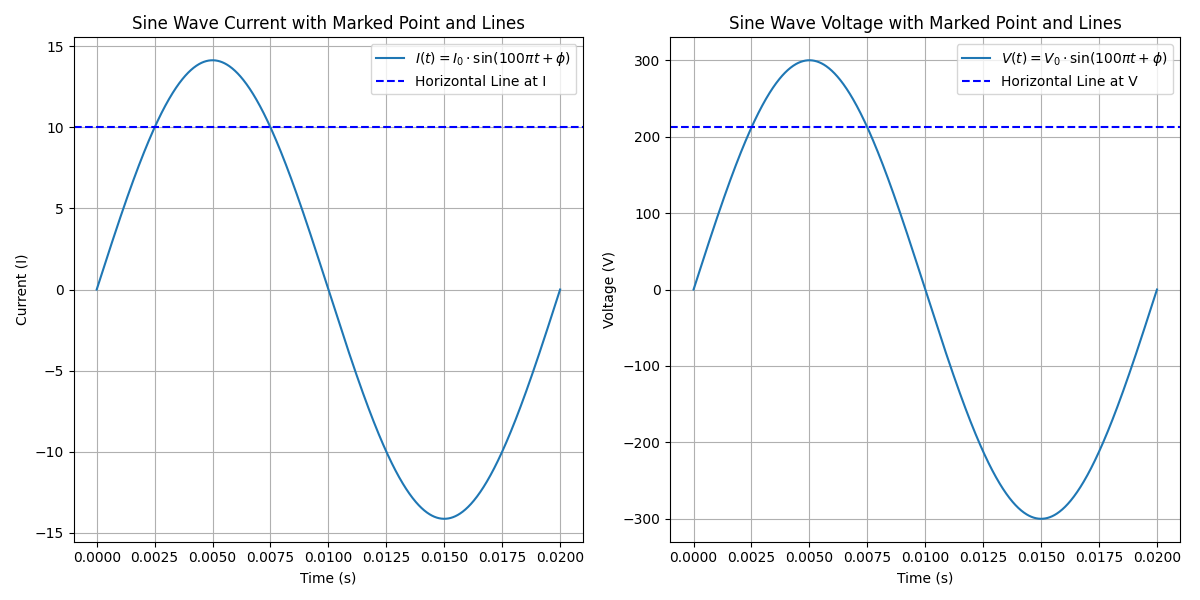
\includegraphics[width=\columnwidth]{ncert-physics/12/7/2/figs/merged_sine_wave_plots.png}

\end{enumerate}
